\chapter{Bibliography: Prerequisites, Usage \& Functionality}
	\section{How to Install and Use the Bibliography Tool}
		The bibliography is created by using \verb|biber|. On a Linux based OS with \verb|TeXlive| as a \LaTeX~backend, it can be installed via the\\[0.125cm]
		\begin{tabular}{ll}
			\verb|texlive-bibtex-extra|& (Debian based distro)\\
			\verb|texlive-bibtexextra|& (Arch based disto)
		\end{tabular}\\
		packages.
		\newline To create the required bibliography files, one has to run in the terminal:\\
		\verb|biber TEXFILENAME|\\
		To update the output pdf accordingly, the following sequence of commands is recommended:\\[-1cm]
		\begin{verbatim}
			pdflatex TEXFILENAME.tex &&
			biber TEXFILENAME &&
			pdflatex TEXFILENAME.tex &&
			pdflatex TEXFILENAME.tex 
		\end{verbatim} 
		\vspace{-0.5cm}
		For \verb|TeXstudio| users, it is possible to select under\\[-1cm]
		\begin{center}
			\verb|Options| $\rightarrow$ 
			\verb|Configure TeXstudio| $\rightarrow$
			\verb|Build|$ \rightarrow$
			\verb|Default Bibliography Tool| 
		\end{center}
		\vspace{-0.5cm}
		\verb|biber| as the default bibliography tool. After that, as soon as a change will occur in any of the bibliography files/data, \verb|TeXstudio| will automatically rebuild the bibliography during the next compilation (so no additional user interaction required). If \verb|TeXstudio| will not do that, a bibliography rebuild can be forced manually by pressing \verb|F8|.
		
	\newpage
	\section{Bibliography and Citation Styles}
		In version \releaseVersion, \verb|minimalthesis| provides the user with two choices for the citation style: \verb|numeric| and \verb|author year|. 
		
		\subsection{{\ttfamily numeric}}
			Per default, \verb|minimalthesis| version \releaseVersion~uses the \verb|numeric| style, which is based upon the \enquote{Angewandte Chemie} (\verb|chem-angew|) bibliography standard.  
			\newline Using this style provides the additional \verb|@arxiv| \cite{arxivExample} and \verb|@thesis| \cite{thesisExample} bibliography drivers, so that Arxiv preprints and theses can be cited properly without any manual adjustments by the user. Their usage is demonstrated in Listing \ref{lst:example-typeset-output-@arxiv-and-@thesis-bib-drivers} and Figure \ref{fig:example-typeset-output-@arxiv-and-@thesis-bib-drivers}.
			
\begin{lstlisting}[
	language={[LaTeX]TeX},
	inputencoding={utf8}, 
	extendedchars=false,  
	escapeinside=``,
	caption={Example bibliography file showing the information required for usage of the {\ttfamily @arxiv} and {\ttfamily @thesis} bibliography drivers provided by {\ttfamily minimalthesis} version \releaseVersion},
	captionpos=b,
	label={lst:example-typeset-output-@arxiv-and-@thesis-bib-drivers}
]
@arxiv{arxivExample,
	title={An Citation Example for Publications on Arxiv},
	author={H. Bartolom`ä`  and L. Murphy},
	year={2023},
	eprint={XXXX.YYYYY},
	archivePrefix={arXiv},
	JOURNALTITLE = {submitted to Journal XYZ, preliminary version 
		        published on arXiv}
}

@thesis{thesisExample,
	author = {J. Doe},
	title={minimalthesis – The Title and a very lengthy Subtitle
	       of the Thesis},
	type = {PhD Thesis},
	institution={University XYZ},
	year={2023}
}	
\end{lstlisting}
			
			\begin{figure}[h!]
				\centering
				\begin{tikzpicture}
					\node[text width=\linewidth, align=center, draw=gray, rectangle, rounded corners=4pt] at (0,0){
						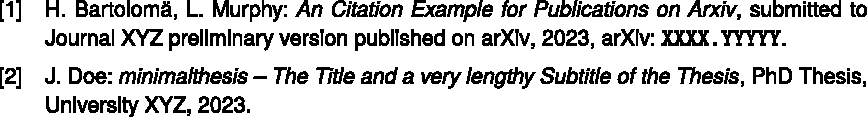
\includegraphics[width=0.975\linewidth]{./quick-start-guide_content/img/minimalthesis_v0-0-2-alpha3_quick-start-guide_arxiv-and-thesis-bib-driver-example.pdf}
					};
				\end{tikzpicture}
				\caption{Example how the {\ttfamily @arxiv} and {\ttfamily @thesis} bibliography drivers provided by {\ttfamily minimalthesis} version \releaseVersion~are typeset in the default configuration.}
				\label{fig:example-typeset-output-@arxiv-and-@thesis-bib-drivers}
			\end{figure}
			
		\newpage
		\subsection{\ttfamily author year}
			By adapting the \verb|bibliography| settings in the \verb|\mtSetupComplete| macro, it is possible to switch from \verb|numeric| to \verb|author year| citation style.
\begin{lstlisting}[
	language={[LaTeX]TeX},
	inputencoding={utf8}, 
	extendedchars=false,  
	escapeinside=``,
	caption={How to change to the {\ttfamily author year} citation style.},
	captionpos=b,
	label={lst:example-author-year-bib-file}
	]
bibliography = {
    style = {
        citing = author year,
        maxcitenames = 1
    },
    file path = ./example-bibliograhy_biber_author-year.bib
}
\end{lstlisting}
		The \verb|maxcitenames| option defines how many other names will be shown, before only the first author followed by \enquote{et al.} will be used as a replacement. If not specified, it defaults to \verb|1|.
		\newline A practical example on how to use the \verb|author year| citation style properly is given with the following paragraphs.
		
\begin{lstlisting}[
	language={[LaTeX]TeX},
	inputencoding={utf8}, 
	extendedchars=false,  
	escapeinside=``,
	caption={Example bibliography file including some example entries specifically tailored to illustrate the functionality and problems of the {\ttfamily author year} citation style.},
	captionpos=b,
	label={lst:example-author-year-bib-file}
	]
@article{testOneAuthor, 
	author = "Tibatong, H.",
	title = "The first Single Author Paper",
	year = "1969"
}

@article{testTwoAuthors, 
	author = "Tibatong, H. and Bartolom`ä` , H.",
	title = "The first Tibatong et Bartolom`ä`  Paper of the Year",
	year = "1969"
}

@article{testThreeAuthors, 
	author = "Tibatong, H. and Bartolom`ä` , H. and Murphy, L.",
	title = "The first Tibatong, Bartolom`ä`  et Murphy Paper of the Year",
	year = "1969"
}

@article{testTwoAuthorsSameYear, 
	author = "Tibatong, H. and Bartolom`ä` , H.",
	title = "The second Tibatong et Bartolom`ä`  Paper of the Year",
	year = "1969"
}
\end{lstlisting}

\begin{lstlisting}[
	language={[LaTeX]TeX},
	inputencoding={utf8}, 
	extendedchars=false,  
	escapeinside=``,
	caption={Example \LaTeX~code to illustrate the functionality and problems of the {\ttfamily author year} citation style. Excerpt from the MWE.},
	captionpos=b,
	label={lst:example-author-year-latex-code}
	]
\chapter{Tests}
    \section{Citations}
        The author year citation works: \cite{testOneAuthor} and \cite{testTwoAuthors}
        and \cite{testThreeAuthors} and \cite{testTwoAuthorsSameYear}. Of course it 
        still has its inherent issues as illustrated above, which is why it should not
        be used for natural science publications and theses.
\end{lstlisting}
		
			\begin{figure}[h!]
				\centering
				\begin{tikzpicture}
					\node[text width=\linewidth, align=center, draw=gray, rectangle, rounded corners=4pt] at (0,0){
						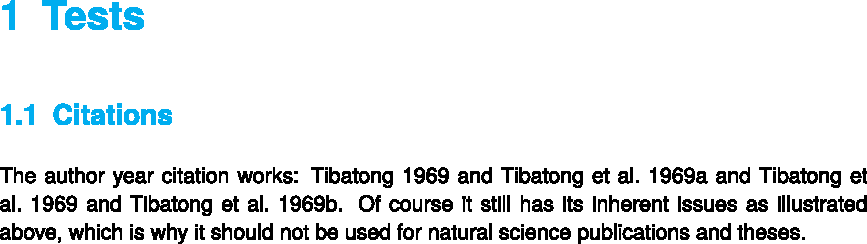
\includegraphics[width=0.975\linewidth]{./quick-start-guide_content/img/minimalthesis_v0-0-2-alpha3_quick-start-guide_author-year-example_text.pdf}
					};
				\end{tikzpicture}
				\caption{Example how the {\ttfamily author year} citation style would look like in a realistic text environment. Excerpt from the MWE.}
				\label{fig:example-typeset-output-author-year-text}
			\end{figure}
			
			\newpage
			\begin{figure}[h!]
				\centering
				\begin{tikzpicture}
					\node[text width=\linewidth, align=center, draw=gray, rectangle, rounded corners=4pt] at (0,0){
						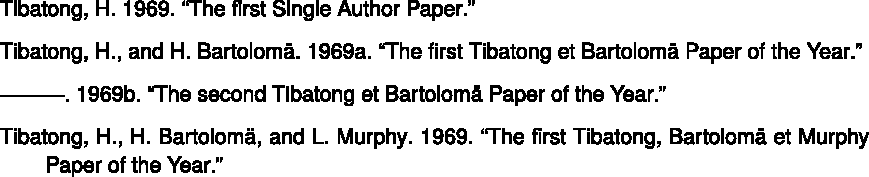
\includegraphics[width=0.975\linewidth]{./quick-start-guide_content/img/minimalthesis_v0-0-2-alpha3_quick-start-guide_author-year-example_bibliography.pdf}
					};
				\end{tikzpicture}
				\caption{Example how the bibliography would look like in the {\ttfamily author year} citation style. Excerpt from the MWE.}
				\label{fig:example-typeset-output-author-year-bib}
			\end{figure}
			
			\subsubsection{Important Notes}
				\begin{itemize}
					\item Changing the citation style from \verb|numeric| to \verb|author year| or vice versa sometimes leads to issues during the first compilation. It is therefor recommended to delete all the auxillary \LaTeX~files before the first compilation with the new setting.
					\item First names of authors have to be abbreviated in bibliography file, otherwise \verb|maxcitenames| does not work properly.
				\end{itemize} 